\documentclass[10pt]{beamer}

%\usepackage[backend=bibtex,firstinits=true,style=verbose-inote,citestyle=authortitle]{biblatex}
\usepackage{bm}
\usepackage{graphicx}
\usepackage{subcaption}
\usepackage{amsmath}
\usepackage{amsfonts}
\usepackage{makecell}
\usepackage{filecontents}
\usepackage{biblatex}
% \newcommand{\expect}[2][]{
\ifthenelse{\equal{#1}{}}{
\mathbb{E}\left[#2\right]
}{
\underset{#1}{\mathbb{E}}\left[#2\right]
}}

\newcommand{\cov}[2][]{
\ifthenelse{\equal{#1}{}}{
\text{Cov}\left[#2\right]
}{
\underset{#1}{\text{Cov}}\left[#2\right]
}}


\newcommand{\var}[2][]{
\ifthenelse{\equal{#1}{}}{
\text{Var}[#2]
}{
\underset{#1}{\text{Var}}[#2]
}}

\newcommand{\loss}[2][]{
\ifthenelse{\equal{#1}{}}{
\mathcal{L}(#2)
}{
\mathcal{L}_{#1}(#2)
}}

\newcommand{\kl}[2]{
\text{D}_\text{KL}[#1 \parallel #2]
}

\newcommand{\R}{\mathbb{R}}
%\newcommand{\Prob}{\mathbb{P}}

\newcommand{\1}[1]{\mathds{1}\{#1\}}


%\usecolortheme{dolphin}
\setbeamertemplate{navigation symbols}{}
\setbeamertemplate{section in toc}{\inserttocsectionnumber.~\inserttocsection}

\begin{filecontents*}{references.bib}
@InProceedings{GLANN,
author = {Hoshen, Yedid and Li, Ke and Malik, Jitendra},
title = {Non-Adversarial Image Synthesis With Generative Latent Nearest Neighbors},
booktitle = {The IEEE Conference on Computer Vision and Pattern Recognition (CVPR)},
month = {June},
year = {2019}
}
\end{filecontents*}

\addbibresource{references.bib}

\title{Non-Adversarial Image Synthesis with Generative Latent Nearest Neighbors\footnote{\citepaper{GLANN}}}
%\subtitle{}
%\author{Ivan Skorokhodov}
%\date{}
%\logo{
\includegraphics[height=1cm]{images/ipavlov-logo.png}}

\newcommand{\citepaper}[1]{\citetitle{#1} by \citeauthor{#1}}

%\graphicspath{{./images}}

%\usetheme{lucid}
\begin{document}

\begin{frame}
    \titlepage
\end{frame}

\begin{frame}{Overview}
    \begin{itemize}
        \item\pause Authors built a ``non-orthodox'' generative model (by merging GLO and IMLE)
        \item\pause They achieved competitive FID/PRD scores and good interpolation properties.
    \end{itemize}
\end{frame}

\begin{frame}{Generative Latent Optimization (GLO)}
    \begin{itemize}
        \item For each image $x_i$ define (randomly) a latent vector $z_i$, s.t. $\| z_i \| = 1$
        \item Define a decoder $G_\theta(z_i) = x_i$.
        \item Optimize both $G_\theta$ and $z_1, ..., z_n$ to minimize
        \begin{equation*}
            \min_{\theta, z_1, ..., z_n} \sum_{i=1}^n \|G_\theta(z_i) - x_i \|_2^2
        \end{equation*}
    \end{itemize}
    
    \begin{figure}
        \centering
        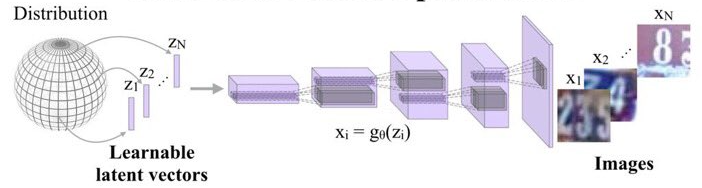
\includegraphics[width=0.8\textwidth]{images/glo}
        \caption{Generative Latent Optimization (GLO) \footnote{The picture by Shao-Hua Sun @shaohua0116}}
    \end{figure}
\end{frame}

\begin{frame}{GLO pros and cons}
    Pros:
    \begin{itemize}
        \item\pause Optimization is simple
        \item\pause Optimization is stable
        \item\pause No mode collapse
    \end{itemize}
    
    Cons:
    \begin{itemize}
        \item\pause Novel samples are bad
        \item\pause We have to store $O(n)$ training latent vectors $z_i$
    \end{itemize}
\end{frame}


\begin{frame}{Implicit Maximum Likelihood Estimation (IMLE)}
    \begin{itemize}
        \item\pause Define a Generator $G_\theta(e) = x$
        \item\pause On each iteration, sample $e \sim \mathcal{N}(0, I)$ and compute $G(e) = \tilde{x}$
        \item\pause Find the closest image $x$ from your dataset and optimize $\| G(e) - x \|_2^2$.
        \item\pause This procedure was shown to be equivalent to MLE.
    \end{itemize}
\end{frame}

\begin{frame}{IMLE pros and cons}
    Pros:
    \begin{itemize}
        \item\pause Idea is simple
        \item\pause Has a theoretical justification
        \item\pause Sampling is easy at test time
    \end{itemize}
    
    Cons:
    \begin{itemize}
        \item\pause $l_2$-nearest neighbour in an image space is costly and not very sensible.
        \item\pause Samples are blurry
    \end{itemize}
\end{frame}


\begin{frame}{Generative Latent Nearest Neighbors (GLANN)}
    \begin{itemize}
        \item\pause Stage 1. Train a GLO model $G:z \to x$ on top of images.
        \item\pause Some details: use perceptual loss instead of Laplacian pyramid to train it.
        \item\pause Stage 2. Train an IMLE model $T:e \to z$ on top of latent vectors.
    \end{itemize}
    
    \begin{figure}
        \centering
        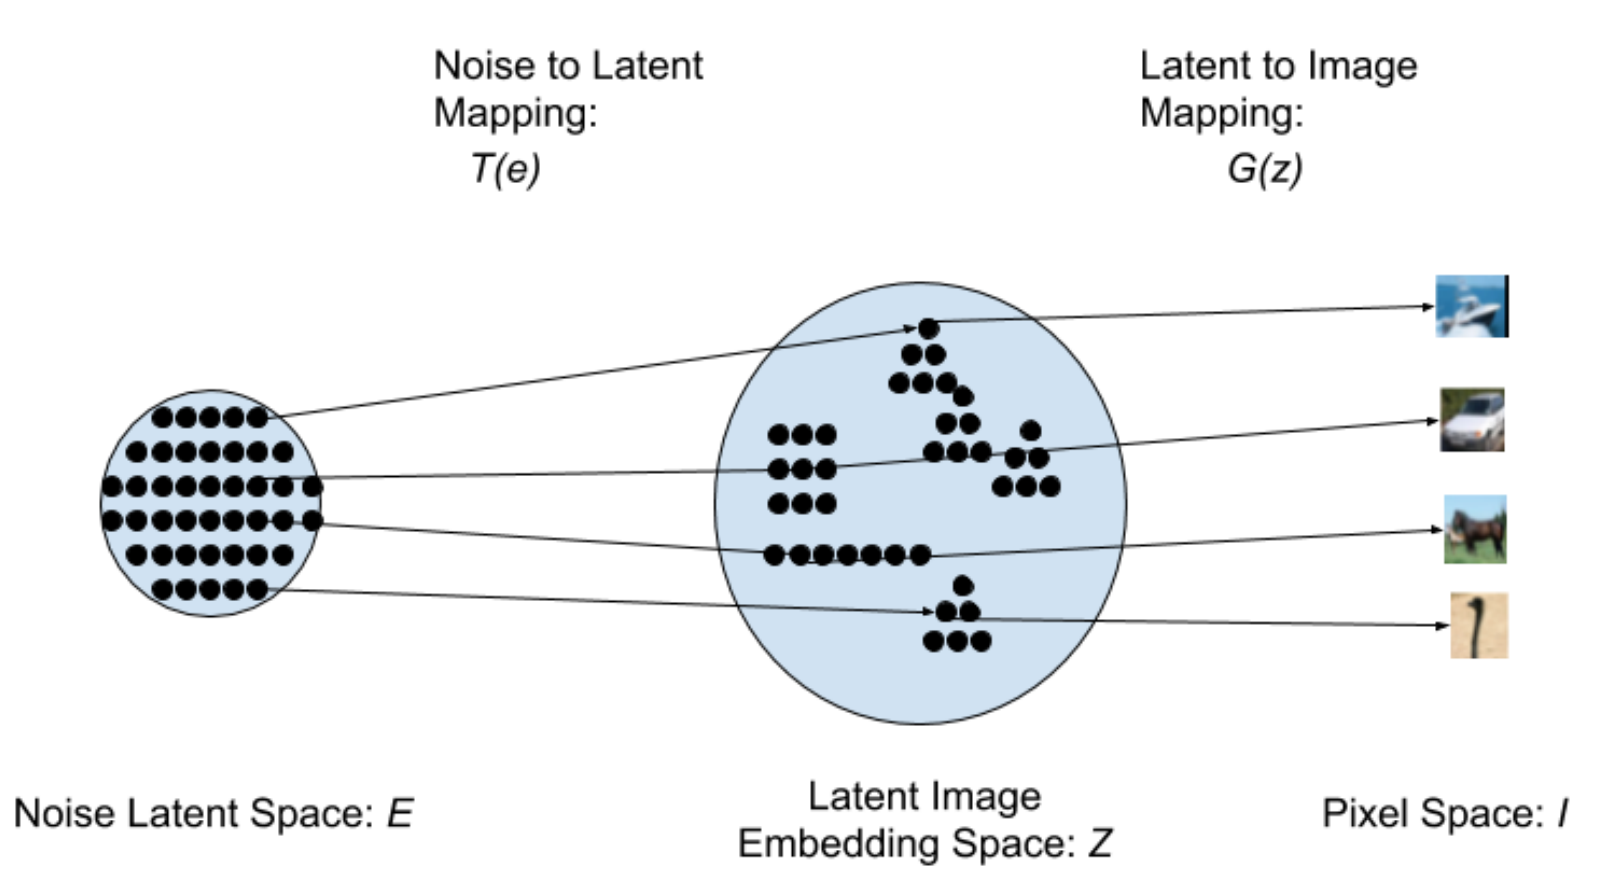
\includegraphics[width=0.8\textwidth]{images/glann}
    \end{figure}
\end{frame}

\begin{frame}{Results}
    \begin{figure}
        \centering
        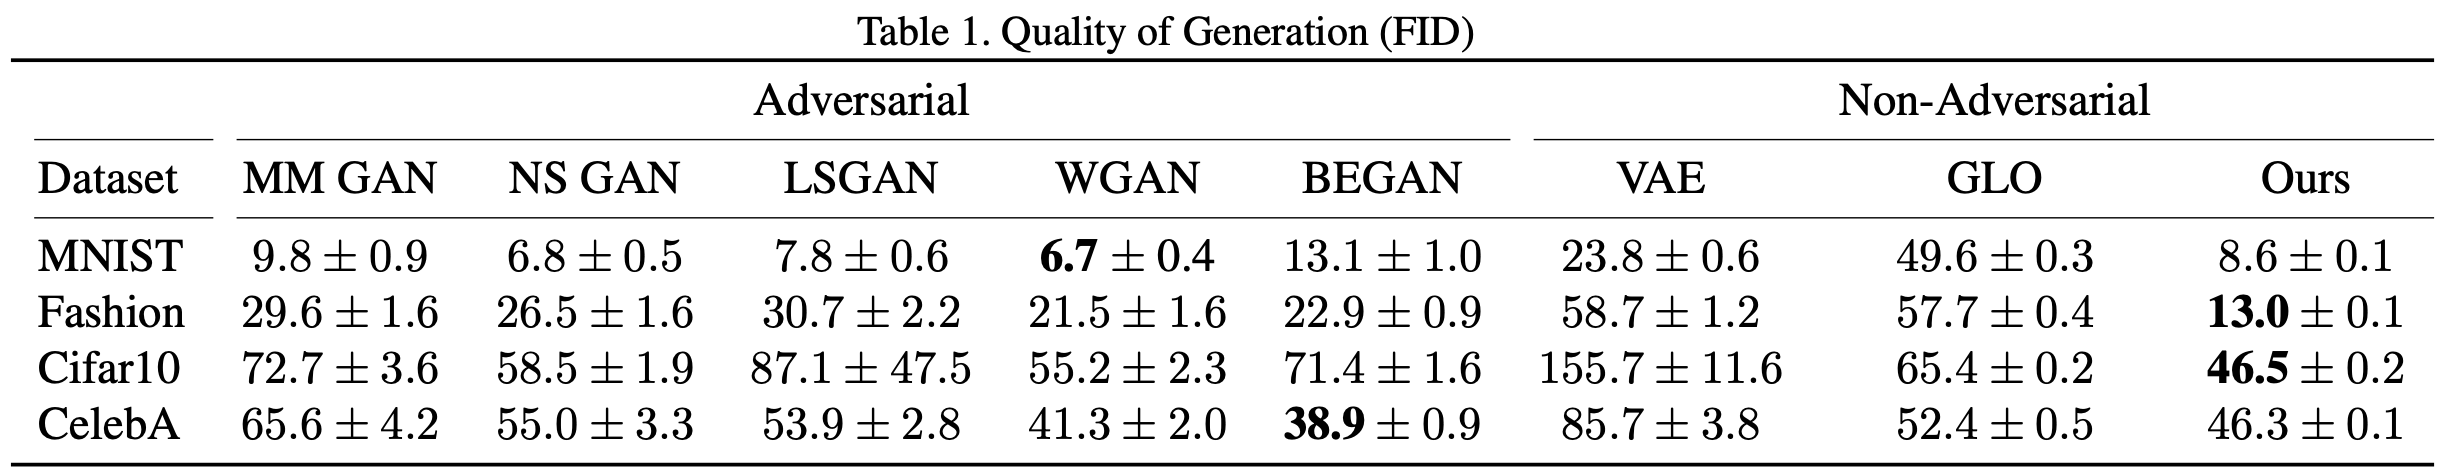
\includegraphics[width=\textwidth]{images/glann-results}
        \caption{GLANN FID scores}
    \end{figure}
    
    \begin{figure}
        \centering
        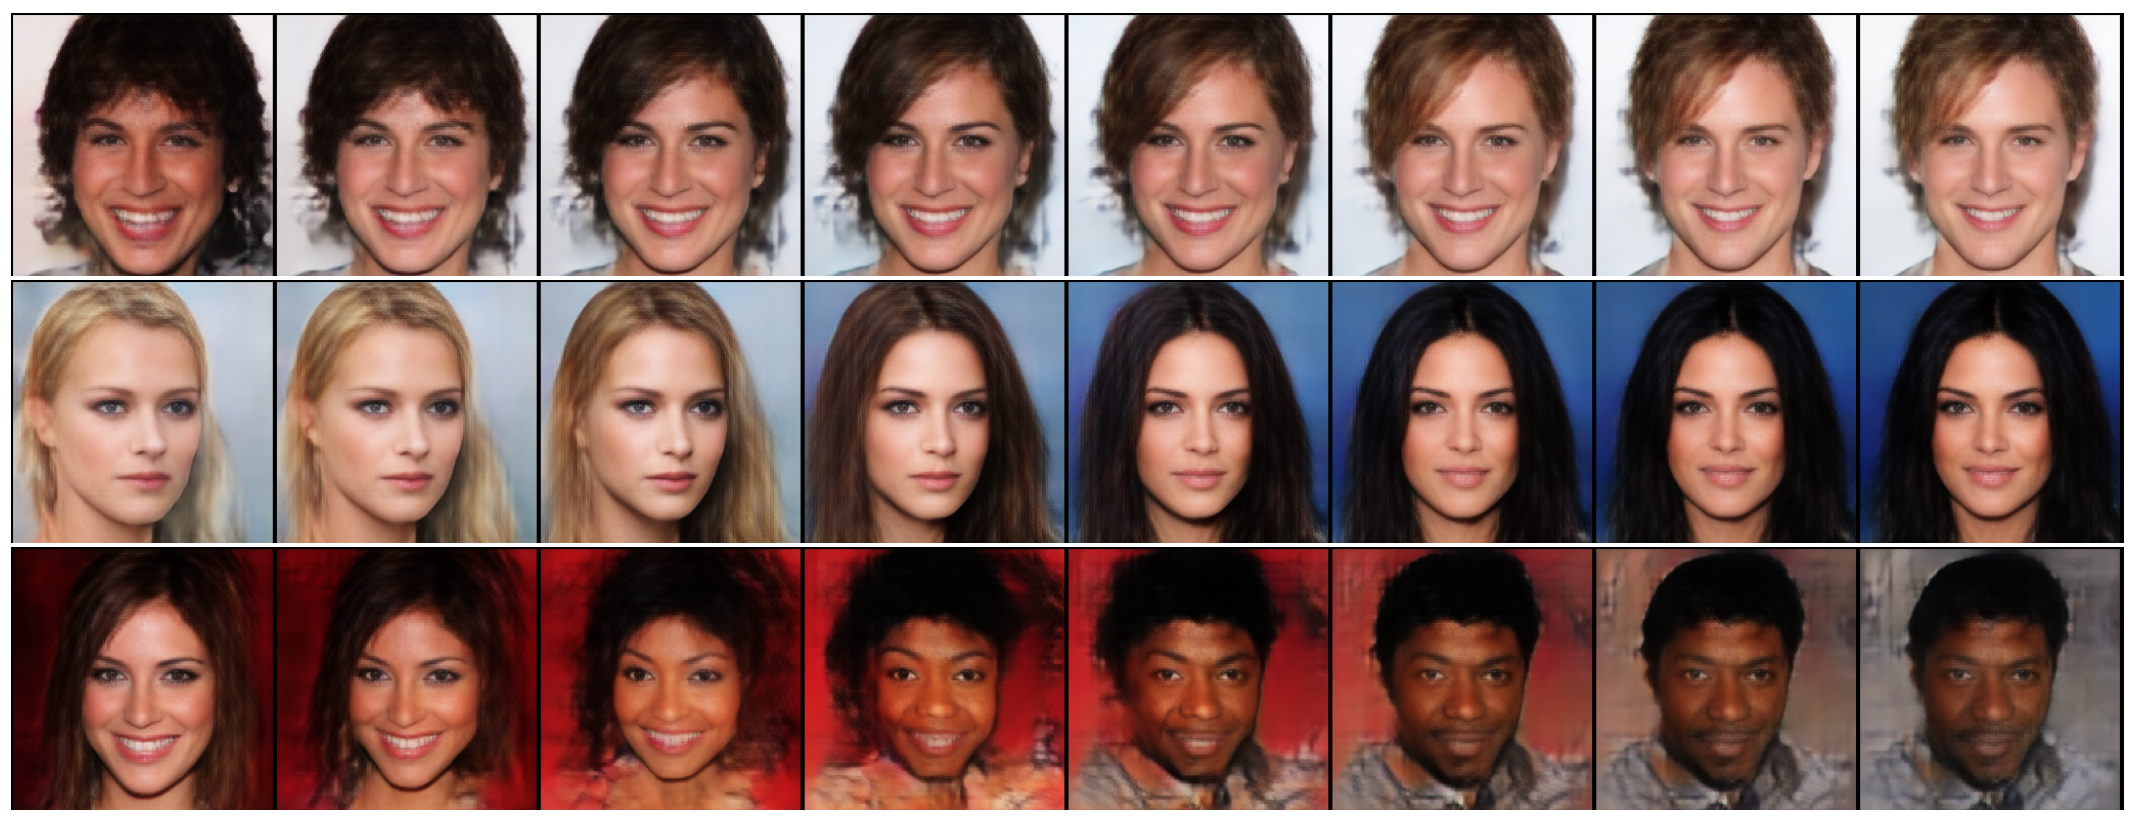
\includegraphics[width=\textwidth]{images/glann-interpolations}
        \caption{GLANN interpolations properties}
    \end{figure}
\end{frame}

\end{document}
